\documentclass[a4paper]{article}
\usepackage{lmodern}
\usepackage{amssymb,amsmath}
\usepackage{ifxetex,ifluatex}
\usepackage{fixltx2e} % provides \textsubscript
\ifnum 0\ifxetex 1\fi\ifluatex 1\fi=0 % if pdftex
  \usepackage[T1]{fontenc}
  \usepackage[utf8]{inputenc}
\else % if luatex or xelatex
  \ifxetex
    \usepackage{mathspec}
  \else
    \usepackage{fontspec}
  \fi
  \defaultfontfeatures{Ligatures=TeX,Scale=MatchLowercase}
    \setmainfont[]{NanumGothic}
\fi
% use upquote if available, for straight quotes in verbatim environments
\IfFileExists{upquote.sty}{\usepackage{upquote}}{}
% use microtype if available
\IfFileExists{microtype.sty}{%
\usepackage{microtype}
\UseMicrotypeSet[protrusion]{basicmath} % disable protrusion for tt fonts
}{}
\usepackage[margin=1in]{geometry}
\usepackage{hyperref}
\hypersetup{unicode=true,
            pdftitle={Carseats - report (Advertising vs Sales)},
            pdfauthor={learningSpoonsDS},
            pdfborder={0 0 0},
            breaklinks=true}
\urlstyle{same}  % don't use monospace font for urls
\usepackage{color}
\usepackage{fancyvrb}
\newcommand{\VerbBar}{|}
\newcommand{\VERB}{\Verb[commandchars=\\\{\}]}
\DefineVerbatimEnvironment{Highlighting}{Verbatim}{commandchars=\\\{\}}
% Add ',fontsize=\small' for more characters per line
\newenvironment{Shaded}{}{}
\newcommand{\KeywordTok}[1]{\textcolor[rgb]{0.00,0.00,1.00}{#1}}
\newcommand{\DataTypeTok}[1]{#1}
\newcommand{\DecValTok}[1]{#1}
\newcommand{\BaseNTok}[1]{#1}
\newcommand{\FloatTok}[1]{#1}
\newcommand{\ConstantTok}[1]{#1}
\newcommand{\CharTok}[1]{\textcolor[rgb]{0.00,0.50,0.50}{#1}}
\newcommand{\SpecialCharTok}[1]{\textcolor[rgb]{0.00,0.50,0.50}{#1}}
\newcommand{\StringTok}[1]{\textcolor[rgb]{0.00,0.50,0.50}{#1}}
\newcommand{\VerbatimStringTok}[1]{\textcolor[rgb]{0.00,0.50,0.50}{#1}}
\newcommand{\SpecialStringTok}[1]{\textcolor[rgb]{0.00,0.50,0.50}{#1}}
\newcommand{\ImportTok}[1]{#1}
\newcommand{\CommentTok}[1]{\textcolor[rgb]{0.00,0.50,0.00}{#1}}
\newcommand{\DocumentationTok}[1]{\textcolor[rgb]{0.00,0.50,0.00}{#1}}
\newcommand{\AnnotationTok}[1]{\textcolor[rgb]{0.00,0.50,0.00}{#1}}
\newcommand{\CommentVarTok}[1]{\textcolor[rgb]{0.00,0.50,0.00}{#1}}
\newcommand{\OtherTok}[1]{\textcolor[rgb]{1.00,0.25,0.00}{#1}}
\newcommand{\FunctionTok}[1]{#1}
\newcommand{\VariableTok}[1]{#1}
\newcommand{\ControlFlowTok}[1]{\textcolor[rgb]{0.00,0.00,1.00}{#1}}
\newcommand{\OperatorTok}[1]{#1}
\newcommand{\BuiltInTok}[1]{#1}
\newcommand{\ExtensionTok}[1]{#1}
\newcommand{\PreprocessorTok}[1]{\textcolor[rgb]{1.00,0.25,0.00}{#1}}
\newcommand{\AttributeTok}[1]{#1}
\newcommand{\RegionMarkerTok}[1]{#1}
\newcommand{\InformationTok}[1]{\textcolor[rgb]{0.00,0.50,0.00}{#1}}
\newcommand{\WarningTok}[1]{\textcolor[rgb]{0.00,0.50,0.00}{\textbf{#1}}}
\newcommand{\AlertTok}[1]{\textcolor[rgb]{1.00,0.00,0.00}{#1}}
\newcommand{\ErrorTok}[1]{\textcolor[rgb]{1.00,0.00,0.00}{\textbf{#1}}}
\newcommand{\NormalTok}[1]{#1}
\usepackage{graphicx,grffile}
\makeatletter
\def\maxwidth{\ifdim\Gin@nat@width>\linewidth\linewidth\else\Gin@nat@width\fi}
\def\maxheight{\ifdim\Gin@nat@height>\textheight\textheight\else\Gin@nat@height\fi}
\makeatother
% Scale images if necessary, so that they will not overflow the page
% margins by default, and it is still possible to overwrite the defaults
% using explicit options in \includegraphics[width, height, ...]{}
\setkeys{Gin}{width=\maxwidth,height=\maxheight,keepaspectratio}
\IfFileExists{parskip.sty}{%
\usepackage{parskip}
}{% else
\setlength{\parindent}{0pt}
\setlength{\parskip}{6pt plus 2pt minus 1pt}
}
\setlength{\emergencystretch}{3em}  % prevent overfull lines
\providecommand{\tightlist}{%
  \setlength{\itemsep}{0pt}\setlength{\parskip}{0pt}}
\setcounter{secnumdepth}{0}
% Redefines (sub)paragraphs to behave more like sections
\ifx\paragraph\undefined\else
\let\oldparagraph\paragraph
\renewcommand{\paragraph}[1]{\oldparagraph{#1}\mbox{}}
\fi
\ifx\subparagraph\undefined\else
\let\oldsubparagraph\subparagraph
\renewcommand{\subparagraph}[1]{\oldsubparagraph{#1}\mbox{}}
\fi

%%% Use protect on footnotes to avoid problems with footnotes in titles
\let\rmarkdownfootnote\footnote%
\def\footnote{\protect\rmarkdownfootnote}

%%% Change title format to be more compact
\usepackage{titling}

% Create subtitle command for use in maketitle
\newcommand{\subtitle}[1]{
  \posttitle{
    \begin{center}\large#1\end{center}
    }
}

\setlength{\droptitle}{-2em}

  \title{Carseats - report (Advertising vs Sales)}
    \pretitle{\vspace{\droptitle}\centering\huge}
  \posttitle{\par}
    \author{learningSpoonsDS}
    \preauthor{\centering\large\emph}
  \postauthor{\par}
      \predate{\centering\large\emph}
  \postdate{\par}
    \date{2018-10-21}


\begin{document}
\maketitle

\subsection{0. Data Import}\label{data-import}

\begin{Shaded}
\begin{Highlighting}[]
\KeywordTok{library}\NormalTok{(dplyr)}
\KeywordTok{library}\NormalTok{(ggplot2)}
\KeywordTok{library}\NormalTok{(ISLR)}
\end{Highlighting}
\end{Shaded}

\begin{Shaded}
\begin{Highlighting}[]
\CommentTok{# str(Carseats)}
\NormalTok{Carseats <-}\StringTok{ }\NormalTok{Carseats }\OperatorTok\StringTok{ }
\StringTok{  }\KeywordTok{filter}\NormalTok{(US }\OperatorTok{==}\StringTok{ "Yes"}\NormalTok{) }\OperatorTok
\StringTok{  }\KeywordTok{filter}\NormalTok{(Advertising }\OperatorTok{!=}\StringTok{ }\DecValTok{0}\NormalTok{)}
\end{Highlighting}
\end{Shaded}

\subsection{1. Basic Plot + Purpose}\label{basic-plot-purpose}

\begin{Shaded}
\begin{Highlighting}[]
\NormalTok{xyPlot <-}\StringTok{ }\KeywordTok{ggplot}\NormalTok{(}\DataTypeTok{data =}\NormalTok{ Carseats, }\KeywordTok{aes}\NormalTok{(}\DataTypeTok{x =}\NormalTok{ Advertising, }\DataTypeTok{y =}\NormalTok{ Sales)) }\OperatorTok{+}
\StringTok{  }\KeywordTok{geom_point}\NormalTok{() }\OperatorTok{+}\StringTok{ }\KeywordTok{stat_smooth}\NormalTok{(}\DataTypeTok{method=}\StringTok{"lm"}\NormalTok{)}
\KeywordTok{print}\NormalTok{(xyPlot)}
\end{Highlighting}
\end{Shaded}

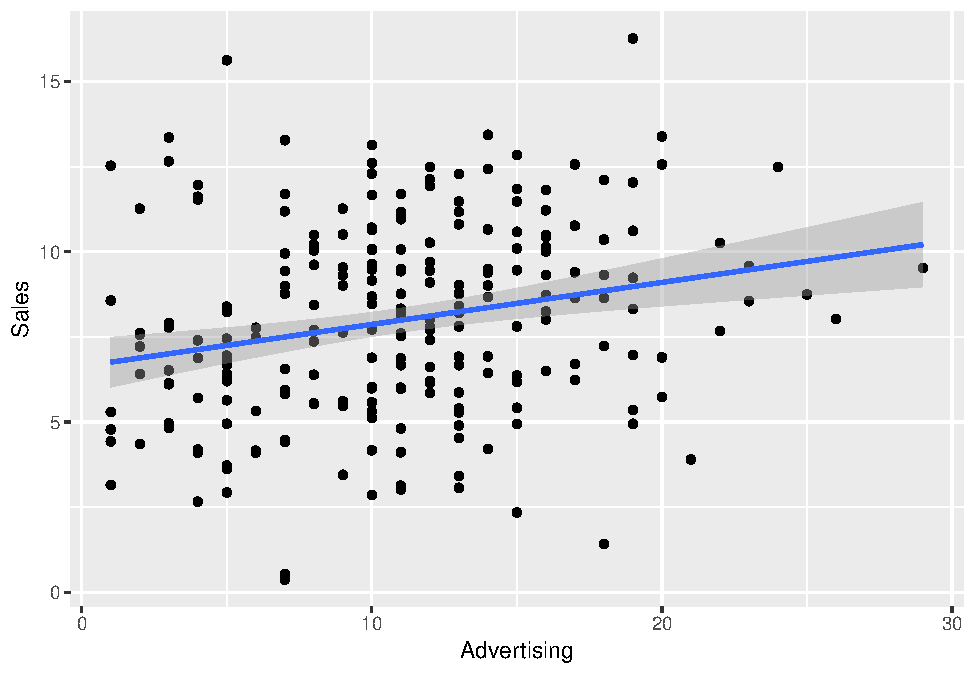
\includegraphics{class3_rmd_pdf_files/figure-latex/unnamed-chunk-3-1.pdf}

\begin{Shaded}
\begin{Highlighting}[]
\CommentTok{# colnames(Carseats)}
\KeywordTok{setdiff}\NormalTok{(}\KeywordTok{colnames}\NormalTok{(Carseats), }\KeywordTok{c}\NormalTok{(}\StringTok{"Sales"}\NormalTok{, }\StringTok{"Advertising"}\NormalTok{))}
\end{Highlighting}
\end{Shaded}

\begin{verbatim}
## [1] "CompPrice"  "Income"     "Population" "Price"      "ShelveLoc" 
## [6] "Age"        "Education"  "Urban"      "US"
\end{verbatim}

\begin{itemize}
\tightlist
\item
  도시 변수에 대해서 광고효과를 알아보는 리포트 입니다.\\
\item
  이 보고서는 \texttt{Advertising}이 \texttt{Sales}에 미치는 영향을
  분석합니다.\\
\item
  Income, Population, Age, Education, Urban, US
\end{itemize}

\begin{enumerate}
\def\labelenumi{\arabic{enumi}.}
\tightlist
\item
  Factor 변수: Urban, US\\
\item
  non-Factor 변수: Income, Population, Age, Education
\end{enumerate}

\begin{itemize}
\tightlist
\item
  후보 추가 변수들은 다음과 같습니다.
  \texttt{setdiff(colnames(Carseats),\ c("Sales",\ "Adverting"))}:
  CompPrice, Income, Advertising, Population, Price, ShelveLoc, Age,
  Education, Urban, US.\\
\item
  각각의 데이터는 각각의 지역 (Spatial Data)를 의미합니다. 그리고
  \texttt{Advertising}와 \texttt{Sales}를 제외한 다른 변수들은 1) 해당
  지역의 특성 혹은 2) 해당 지역에서의 business practice의 특성을
  반영합니다. (factor 변수는 bold로 표기하였습니다.)\\
\end{itemize}

\begin{enumerate}
\def\labelenumi{\arabic{enumi}.}
\tightlist
\item
  해당 지역의 특성: \texttt{Income}, \texttt{Population}, \texttt{Age},
  \texttt{Education}, \textbf{\texttt{Urban}}, \textbf{\texttt{US}}\\
\item
  해당 지역의 biz의 특성: \texttt{CompPrice}, \texttt{Price},
  \textbf{\texttt{ShelveLoc}}
\end{enumerate}

\begin{itemize}
\tightlist
\item
  해당 지역의 특성에 따라서 광고 효과를 살펴봅니다.\\
\end{itemize}

\begin{enumerate}
\def\labelenumi{\arabic{enumi}.}
\tightlist
\item
  Factor 변수에 따라서 광고 효과가 달라지는지 살펴봅니다.\\
\item
  Factor 변수가 아닌 경우에는 4분위 값을 기준으로 Factor 변수로 변환하여
  살펴봅니다.
\end{enumerate}

\subsection{2. Factor 변수 분석}\label{factor--}

\begin{Shaded}
\begin{Highlighting}[]
\NormalTok{xyPlot }\OperatorTok{+}\StringTok{ }\KeywordTok{facet_wrap}\NormalTok{(}\OperatorTok{~}\StringTok{ }\NormalTok{Urban) }\OperatorTok{+}\StringTok{ }\KeywordTok{ggtitle}\NormalTok{(}\StringTok{"by Urban"}\NormalTok{) }\OperatorTok{+}\StringTok{ }\KeywordTok{stat_smooth}\NormalTok{(}\DataTypeTok{method=}\StringTok{"lm"}\NormalTok{)}
\end{Highlighting}
\end{Shaded}

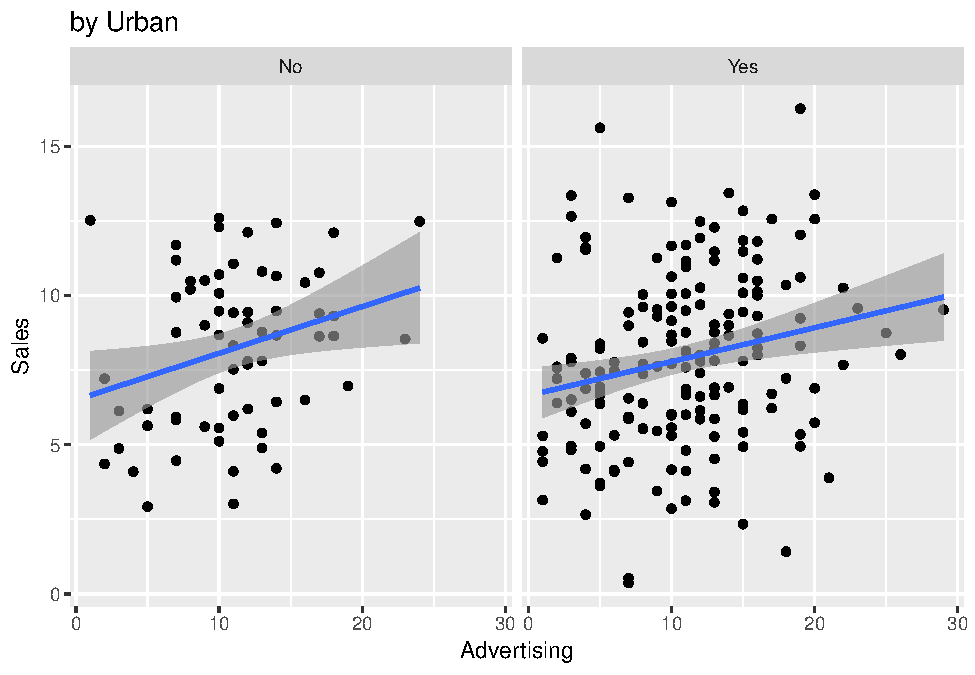
\includegraphics{class3_rmd_pdf_files/figure-latex/unnamed-chunk-5-1.pdf}

\begin{Shaded}
\begin{Highlighting}[]
\NormalTok{xyPlot }\OperatorTok{+}\StringTok{ }\KeywordTok{facet_wrap}\NormalTok{(}\OperatorTok{~}\StringTok{ }\NormalTok{US) }\OperatorTok{+}\StringTok{ }\KeywordTok{ggtitle}\NormalTok{(}\StringTok{"by US"}\NormalTok{) }\OperatorTok{+}\StringTok{ }\KeywordTok{stat_smooth}\NormalTok{(}\DataTypeTok{method=}\StringTok{"lm"}\NormalTok{)}
\end{Highlighting}
\end{Shaded}

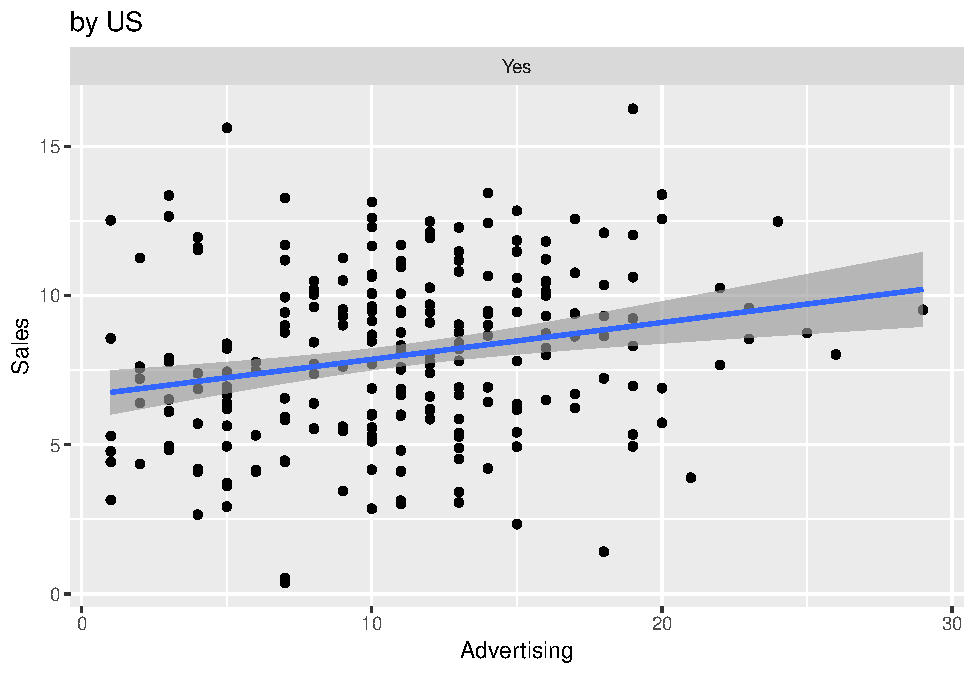
\includegraphics{class3_rmd_pdf_files/figure-latex/unnamed-chunk-5-2.pdf}

\subsection{3. Non-Factor 변수 분석}\label{non-factor--}

\paragraph{1. Mutate Factors}\label{mutate-factors}

\textbf{Method 1 - basic method}

\begin{Shaded}
\begin{Highlighting}[]
\NormalTok{Carseats <-}\StringTok{ }\NormalTok{Carseats }\OperatorTok
\StringTok{  }\KeywordTok{mutate}\NormalTok{(}
    \DataTypeTok{IncomeF =} 
      \KeywordTok{ifelse}\NormalTok{(Income }\OperatorTok{<}\StringTok{ }\KeywordTok{summary}\NormalTok{(Carseats}\OperatorTok{$}\NormalTok{Income)[}\DecValTok{2}\NormalTok{], }\StringTok{"Q1"}\NormalTok{,}
             \KeywordTok{ifelse}\NormalTok{(Income }\OperatorTok{<}\StringTok{ }\KeywordTok{summary}\NormalTok{(Carseats}\OperatorTok{$}\NormalTok{Income)[}\DecValTok{3}\NormalTok{], }\StringTok{"Q2"}\NormalTok{,}
                    \KeywordTok{ifelse}\NormalTok{(Income }\OperatorTok{<}\StringTok{ }\KeywordTok{summary}\NormalTok{(Carseats}\OperatorTok{$}\NormalTok{Income)[}\DecValTok{5}\NormalTok{], }\StringTok{"Q3"}\NormalTok{, }\StringTok{"Q4"}\NormalTok{)))) }\OperatorTok
\StringTok{  }\KeywordTok{mutate}\NormalTok{(}
    \DataTypeTok{AgeF =} 
      \KeywordTok{ifelse}\NormalTok{(Age }\OperatorTok{<}\StringTok{ }\KeywordTok{summary}\NormalTok{(Carseats}\OperatorTok{$}\NormalTok{Age)[}\DecValTok{2}\NormalTok{], }\StringTok{"Q1"}\NormalTok{,}
             \KeywordTok{ifelse}\NormalTok{(Age }\OperatorTok{<}\StringTok{ }\KeywordTok{summary}\NormalTok{(Carseats}\OperatorTok{$}\NormalTok{Age)[}\DecValTok{3}\NormalTok{], }\StringTok{"Q2"}\NormalTok{,}
                    \KeywordTok{ifelse}\NormalTok{(Age }\OperatorTok{<}\StringTok{ }\KeywordTok{summary}\NormalTok{(Carseats}\OperatorTok{$}\NormalTok{Age)[}\DecValTok{5}\NormalTok{], }\StringTok{"Q3"}\NormalTok{, }\StringTok{"Q4"}\NormalTok{))))  }
\end{Highlighting}
\end{Shaded}

\textbf{Method 2 - using function}

\begin{Shaded}
\begin{Highlighting}[]
\NormalTok{generateQuartile <-}\StringTok{ }\ControlFlowTok{function}\NormalTok{(x) \{}
  \KeywordTok{return}\NormalTok{(}\KeywordTok{summary}\NormalTok{(x)[}\KeywordTok{c}\NormalTok{(}\DecValTok{2}\NormalTok{,}\DecValTok{3}\NormalTok{,}\DecValTok{5}\NormalTok{)])}
\NormalTok{\}}
\NormalTok{Carseats <-}\StringTok{ }\NormalTok{Carseats }\OperatorTok
\StringTok{  }\KeywordTok{mutate}\NormalTok{(}
    \DataTypeTok{IncomeF =} 
      \KeywordTok{ifelse}\NormalTok{(Income }\OperatorTok{<}\StringTok{ }\KeywordTok{generateQuartile}\NormalTok{(Carseats}\OperatorTok{$}\NormalTok{Income)[}\DecValTok{1}\NormalTok{], }\StringTok{"Q1"}\NormalTok{,}
             \KeywordTok{ifelse}\NormalTok{(Income }\OperatorTok{<}\StringTok{ }\KeywordTok{generateQuartile}\NormalTok{(Carseats}\OperatorTok{$}\NormalTok{Income)[}\DecValTok{2}\NormalTok{], }\StringTok{"Q2"}\NormalTok{,}
                    \KeywordTok{ifelse}\NormalTok{(Income }\OperatorTok{<}\StringTok{ }\KeywordTok{generateQuartile}\NormalTok{(Carseats}\OperatorTok{$}\NormalTok{Income)[}\DecValTok{3}\NormalTok{], }\StringTok{"Q3"}\NormalTok{, }\StringTok{"Q4"}\NormalTok{)))) }\OperatorTok
\StringTok{  }\KeywordTok{mutate}\NormalTok{(}
    \DataTypeTok{AgeF =} 
      \KeywordTok{ifelse}\NormalTok{(Age }\OperatorTok{<}\StringTok{ }\KeywordTok{generateQuartile}\NormalTok{(Carseats}\OperatorTok{$}\NormalTok{Age)[}\DecValTok{1}\NormalTok{], }\StringTok{"Q1"}\NormalTok{,}
             \KeywordTok{ifelse}\NormalTok{(Age }\OperatorTok{<}\StringTok{ }\KeywordTok{generateQuartile}\NormalTok{(Carseats}\OperatorTok{$}\NormalTok{Age)[}\DecValTok{2}\NormalTok{], }\StringTok{"Q2"}\NormalTok{,}
                    \KeywordTok{ifelse}\NormalTok{(Age }\OperatorTok{<}\StringTok{ }\KeywordTok{generateQuartile}\NormalTok{(Carseats}\OperatorTok{$}\NormalTok{Age)[}\DecValTok{3}\NormalTok{], }\StringTok{"Q3"}\NormalTok{, }\StringTok{"Q4"}\NormalTok{)))) }\OperatorTok\StringTok{  }
\StringTok{  }\KeywordTok{mutate}\NormalTok{(}
    \DataTypeTok{EducationF =} 
      \KeywordTok{ifelse}\NormalTok{(Education }\OperatorTok{<}\StringTok{ }\KeywordTok{generateQuartile}\NormalTok{(Carseats}\OperatorTok{$}\NormalTok{Education)[}\DecValTok{1}\NormalTok{], }\StringTok{"Q1"}\NormalTok{,}
             \KeywordTok{ifelse}\NormalTok{(Education }\OperatorTok{<}\StringTok{ }\KeywordTok{generateQuartile}\NormalTok{(Carseats}\OperatorTok{$}\NormalTok{Education)[}\DecValTok{2}\NormalTok{], }\StringTok{"Q2"}\NormalTok{,}
                    \KeywordTok{ifelse}\NormalTok{(Education }\OperatorTok{<}\StringTok{ }\KeywordTok{generateQuartile}\NormalTok{(Carseats}\OperatorTok{$}\NormalTok{Education)[}\DecValTok{3}\NormalTok{], }\StringTok{"Q3"}\NormalTok{, }\StringTok{"Q4"}\NormalTok{)))) }\OperatorTok
\StringTok{  }\KeywordTok{mutate}\NormalTok{(}
    \DataTypeTok{PopulationF =} 
      \KeywordTok{ifelse}\NormalTok{(Population }\OperatorTok{<}\StringTok{ }\KeywordTok{generateQuartile}\NormalTok{(Carseats}\OperatorTok{$}\NormalTok{Population)[}\DecValTok{1}\NormalTok{], }\StringTok{"Q1"}\NormalTok{,}
             \KeywordTok{ifelse}\NormalTok{(Population }\OperatorTok{<}\StringTok{ }\KeywordTok{generateQuartile}\NormalTok{(Carseats}\OperatorTok{$}\NormalTok{Population)[}\DecValTok{2}\NormalTok{], }\StringTok{"Q2"}\NormalTok{,}
                    \KeywordTok{ifelse}\NormalTok{(Population }\OperatorTok{<}\StringTok{ }\KeywordTok{generateQuartile}\NormalTok{(Carseats}\OperatorTok{$}\NormalTok{Population)[}\DecValTok{3}\NormalTok{], }\StringTok{"Q3"}\NormalTok{, }\StringTok{"Q4"}\NormalTok{))))}
\end{Highlighting}
\end{Shaded}

\paragraph{2. Draw Plots}\label{draw-plots}

\textbf{Method 1 - basic method}

\begin{Shaded}
\begin{Highlighting}[]
\NormalTok{xyPlot <-}\StringTok{ }\KeywordTok{ggplot}\NormalTok{(Carseats, }\KeywordTok{aes}\NormalTok{(}\DataTypeTok{x =}\NormalTok{ Advertising, }\DataTypeTok{y =}\NormalTok{ Sales)) }\OperatorTok{+}
\StringTok{  }\KeywordTok{geom_point}\NormalTok{() }\OperatorTok{+}\StringTok{ }\KeywordTok{stat_smooth}\NormalTok{(}\DataTypeTok{method=}\StringTok{"lm"}\NormalTok{) }
  \CommentTok{# Let xyPlot to update the dataset  }
\NormalTok{xyPlot }\OperatorTok{+}\StringTok{ }\KeywordTok{facet_wrap}\NormalTok{(}\OperatorTok{~}\StringTok{ }\NormalTok{IncomeF) }\OperatorTok{+}\StringTok{ }\KeywordTok{ggtitle}\NormalTok{(}\StringTok{"by Income"}\NormalTok{) }\OperatorTok{+}
\StringTok{  }\KeywordTok{labs}\NormalTok{(}\DataTypeTok{subtitle =} \KeywordTok{generateQuartile}\NormalTok{(Carseats}\OperatorTok{$}\NormalTok{Income) }\OperatorTok\StringTok{ }\KeywordTok{paste}\NormalTok{(}\DataTypeTok{collapse =} \StringTok{","}\NormalTok{))}
\NormalTok{xyPlot }\OperatorTok{+}\StringTok{ }\KeywordTok{facet_wrap}\NormalTok{(}\OperatorTok{~}\StringTok{ }\NormalTok{AgeF) }\OperatorTok{+}\StringTok{ }\KeywordTok{ggtitle}\NormalTok{(}\StringTok{"by Age"}\NormalTok{) }\OperatorTok{+}
\StringTok{  }\KeywordTok{labs}\NormalTok{(}\DataTypeTok{subtitle =} \KeywordTok{generateQuartile}\NormalTok{(Carseats}\OperatorTok{$}\NormalTok{Age) }\OperatorTok\StringTok{ }\KeywordTok{paste}\NormalTok{(}\DataTypeTok{collapse =} \StringTok{","}\NormalTok{))}
\NormalTok{xyPlot }\OperatorTok{+}\StringTok{ }\KeywordTok{facet_wrap}\NormalTok{(}\OperatorTok{~}\StringTok{ }\NormalTok{EducationF) }\OperatorTok{+}\StringTok{ }\KeywordTok{ggtitle}\NormalTok{(}\StringTok{"by Education"}\NormalTok{) }\OperatorTok{+}\StringTok{ }
\StringTok{  }\KeywordTok{labs}\NormalTok{(}\DataTypeTok{subtitle =} \KeywordTok{generateQuartile}\NormalTok{(Carseats}\OperatorTok{$}\NormalTok{Education) }\OperatorTok\StringTok{ }\KeywordTok{paste}\NormalTok{(}\DataTypeTok{collapse =} \StringTok{","}\NormalTok{))}
\NormalTok{xyPlot }\OperatorTok{+}\StringTok{ }\KeywordTok{facet_wrap}\NormalTok{(}\OperatorTok{~}\StringTok{ }\NormalTok{PopulationF) }\OperatorTok{+}\StringTok{ }\KeywordTok{ggtitle}\NormalTok{(}\StringTok{"by Population"}\NormalTok{) }\OperatorTok{+}
\StringTok{  }\KeywordTok{labs}\NormalTok{(}\DataTypeTok{subtitle =} \KeywordTok{generateQuartile}\NormalTok{(Carseats}\OperatorTok{$}\NormalTok{Population) }\OperatorTok\StringTok{ }\KeywordTok{paste}\NormalTok{(}\DataTypeTok{collapse =} \StringTok{","}\NormalTok{))}
\end{Highlighting}
\end{Shaded}

\textbf{Method 2 - advanced - using for loop}

\begin{itemize}
\tightlist
\item
  Variable의 갯수에 많아져도 코드가 길어지지 않도록 처리합니다.\\
\item
  반복문 안에서
  \texttt{facet\_wrap(as.formula(paste0("\textasciitilde{}",\ var,\ "F")))}를
  사용하여 string 값인 \texttt{var}를 변수 입력으로 사용할 수
  있습니다.\\
\item
  같은 목적으로
  \texttt{generateQuartile(eval(parse(text=paste0("Carseats\$",\ var))))}를
  사용하여 \texttt{var}를 변수 입력으로 사용할 수 있습니다.
\end{itemize}

\begin{Shaded}
\begin{Highlighting}[]
\NormalTok{xyPlot <-}\StringTok{ }
\StringTok{  }\KeywordTok{ggplot}\NormalTok{(}\DataTypeTok{data =}\NormalTok{ Carseats, }\KeywordTok{aes}\NormalTok{(}\DataTypeTok{x =}\NormalTok{ Advertising, }\DataTypeTok{y =}\NormalTok{ Sales)) }\OperatorTok{+}\StringTok{ }
\StringTok{  }\KeywordTok{geom_point}\NormalTok{() }\OperatorTok{+}\StringTok{ }\KeywordTok{stat_smooth}\NormalTok{(}\DataTypeTok{method=}\StringTok{"lm"}\NormalTok{) }
  \CommentTok{# Let xyPlot to update the dataset   }
\NormalTok{variables <-}\StringTok{ }\KeywordTok{c}\NormalTok{(}\StringTok{"Income"}\NormalTok{, }\StringTok{"Population"}\NormalTok{, }\StringTok{"Age"}\NormalTok{, }\StringTok{"Education"}\NormalTok{)}
\ControlFlowTok{for}\NormalTok{ (var }\ControlFlowTok{in}\NormalTok{ variables) \{}
\NormalTok{  a <-}\StringTok{ }\NormalTok{xyPlot }\OperatorTok{+}\StringTok{ }
\StringTok{    }\KeywordTok{facet_wrap}\NormalTok{(}\KeywordTok{as.formula}\NormalTok{(}\KeywordTok{paste0}\NormalTok{(}\StringTok{"~"}\NormalTok{, var, }\StringTok{"F"}\NormalTok{))) }\OperatorTok{+}
\StringTok{    }\KeywordTok{labs}\NormalTok{(}\DataTypeTok{title =} 
           \KeywordTok{paste0}\NormalTok{(}\StringTok{"by "}\NormalTok{, var, }\StringTok{"F"}\NormalTok{),}
         \DataTypeTok{subtitle =} 
           \KeywordTok{generateQuartile}\NormalTok{(}\KeywordTok{eval}\NormalTok{(}\KeywordTok{parse}\NormalTok{(}\DataTypeTok{text=}\KeywordTok{paste0}\NormalTok{(}\StringTok{"Carseats$"}\NormalTok{, var)))) }\OperatorTok
\StringTok{           }\KeywordTok{as.numeric}\NormalTok{() }\OperatorTok\StringTok{ }\KeywordTok{paste}\NormalTok{(}\DataTypeTok{collapse =} \StringTok{","}\NormalTok{))}
  \KeywordTok{print}\NormalTok{(a)}
\NormalTok{\}}
\end{Highlighting}
\end{Shaded}

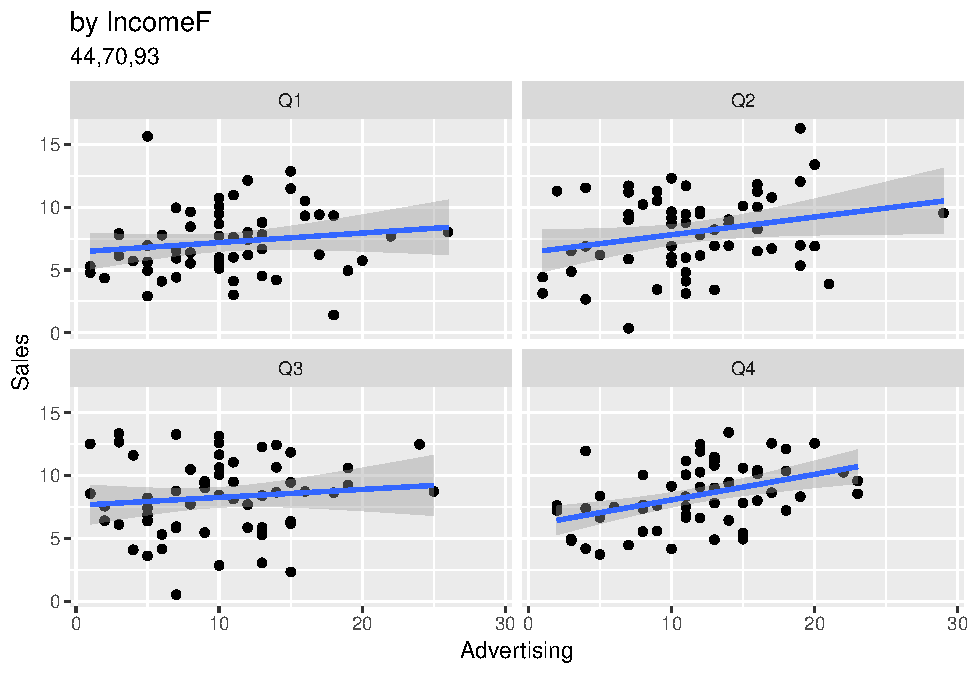
\includegraphics{class3_rmd_pdf_files/figure-latex/unnamed-chunk-9-1.pdf}
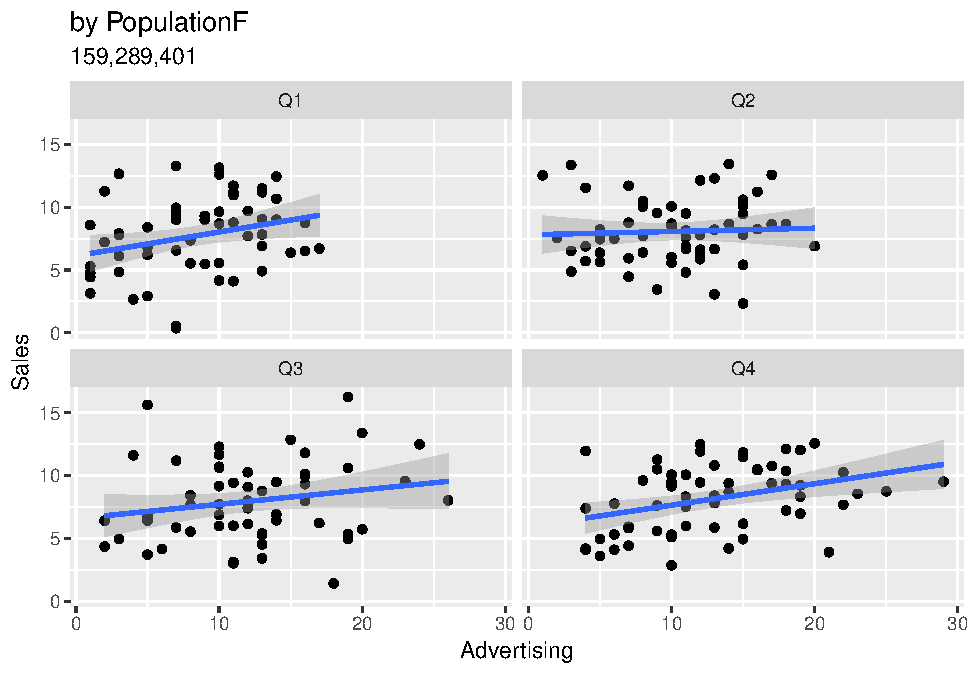
\includegraphics{class3_rmd_pdf_files/figure-latex/unnamed-chunk-9-2.pdf}
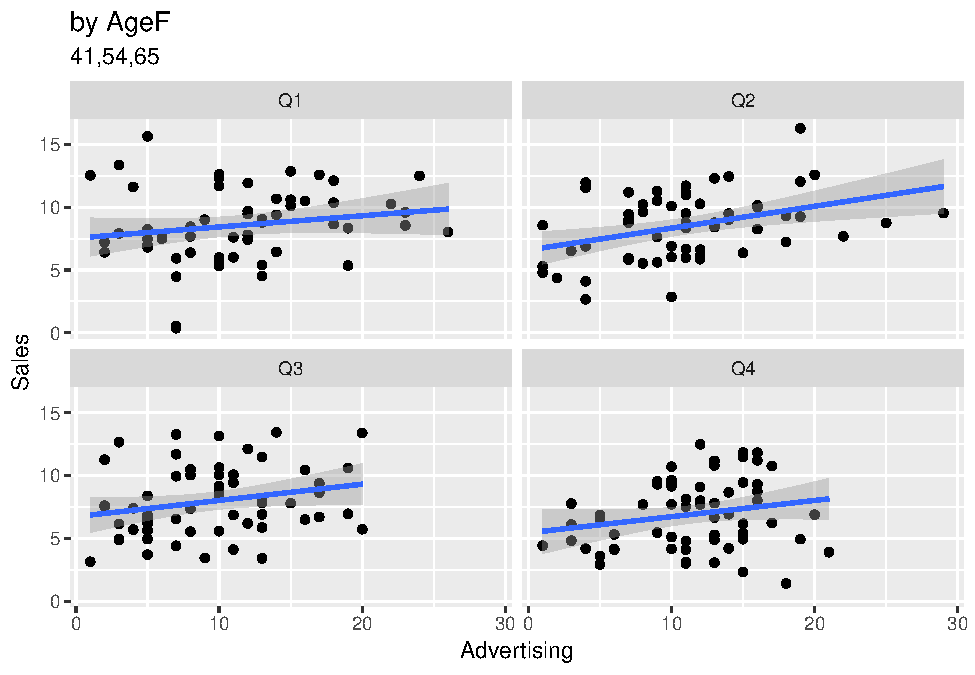
\includegraphics{class3_rmd_pdf_files/figure-latex/unnamed-chunk-9-3.pdf}
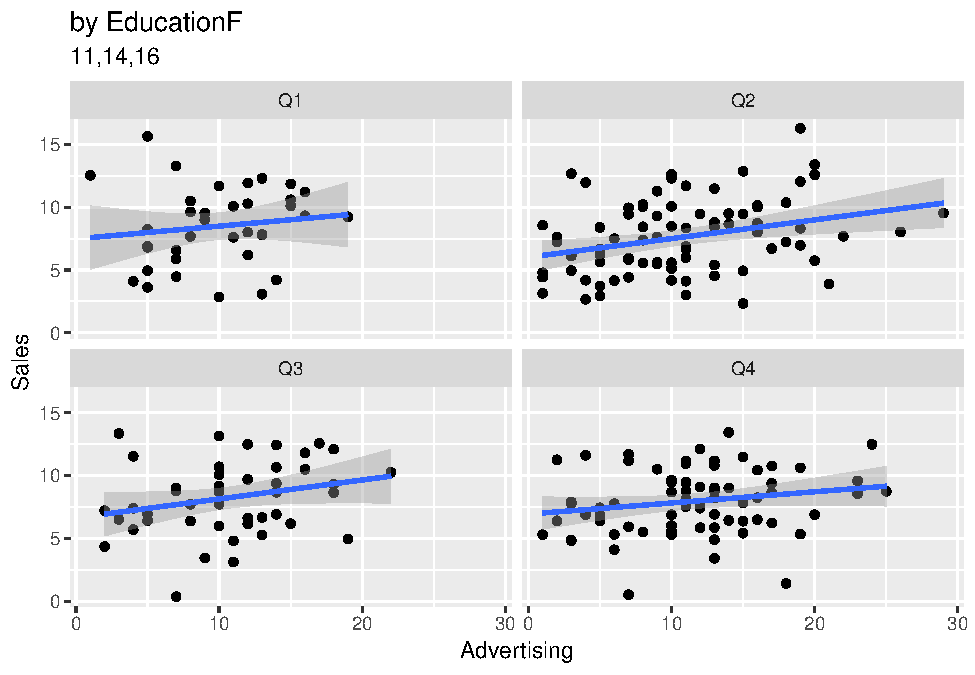
\includegraphics{class3_rmd_pdf_files/figure-latex/unnamed-chunk-9-4.pdf}


\end{document}
